% Bagian Analisis Hasil Percobaan
    
\section*{Analisis Hasil Percobaan}
\indent
Pada praktikum hari kedua kelompok 17 akan melaksanakan tugas modul 2 yaitu membuat desain schematic dan PCB yang nantinya akan di print. Software yang digunakan untuk praktikum kali ini bernama Autodesk Fusion. Yang harus peserta perhatikan saat membuat desain ini adalah ketika akan menyambungkan tiap komponen menggunakan jalur yang nantinya akan di print di PCB. Jalur pada PCB tidak boleh saling bertabrakan, berdempetan terlalu dekat ataupun tidak menyambung dengan benar. Salah satu solusi ketika jalur yang digunakan bertabrakan adalah dengan menggunakan layer lain. Karena PCB memiliki 2 sisi kita bisa memanfaatkan kedua sisi itu untuk membuat jalur yang dihubungkan dengan lubang Vias.

\begin{figure}[H]
    \centering
    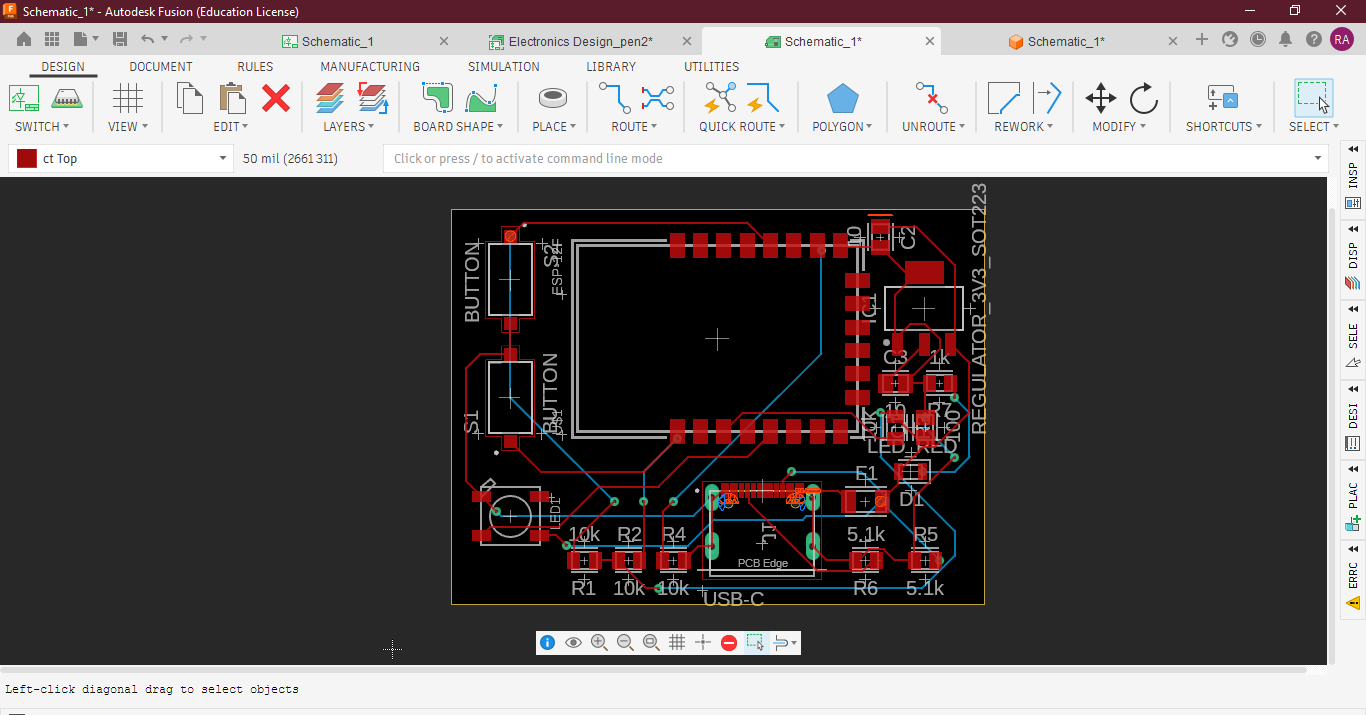
\includegraphics[width=\linewidth]{img/pcb_route.png}
    \caption{Gambar desain PCB.} 
    \label{fig:ini2}
\end{figure}

\subsection*{Langkah untuk mendesain PCB}
\begin{enumerate}
    \item Setelah membuat schematic sebagai tugas pendahuluan, selanjutnya peserta lanjut membuat desain PCBnya sesuai dengan modul yang diberikan.
    \item dengan mengklik tombol 2D PCB di kiri atas.
    \begin{figure}[H]
        \centering
        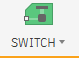
\includegraphics[width=0.5\linewidth]{img/2dpcb.png}
        \caption{Gambar Tombol Untuk Mendesain PCB.} 
        \label{fig:ini3}
    \end{figure}
    \item Setelah tampil wujud dari komponen-komponen dari pcb. Yang peserta lakukan selanjutnya adalah menyambungkan setiap komponen yang memiliki garis kuning pada titiknya ke titik lainnya.
    \item Setelah tersambung semua titiknya, peserta meminta pendapat apakah hasil kerjanya sudah dilakukan dengan baik ke pendamping praktik di lab.
    \item Setelah memastikan dengan benar semua komponen telah disambungkan dengan benar dan baik, peserta mendapatkan tantangan membuat PCB berbentuk bola lampu.
    \item Akhirnya praktik hari ini berhenti dengan hasil berikut.
\end{enumerate}


% \begin{table}[h]
%     \centering
%     \caption{Caption tabelnya}
%     \label{tab:labelini}
%     \begin{tabular}{|c|c|c|}
%         \hline
%         Kolom 1 & Kolom 2 & Kolom 3 \\
%         \hline
%         Data 1 & Data 2 & Data 3 \\
%         Data 4 & Data 5 & Data 6 \\
%         \hline
%     \end{tabular}
% \end{table}